% This is added to allow editing only this part of the document
\documentclass[A4,12pt,oneside]{article}
%A4,12pt,titlepage,oneside,final

% list of packages
\usepackage[a4paper,left=2cm,right=2cm,top=2cm,bottom=2cm]{geometry} % document size

\usepackage[utf8]{inputenc}
\usepackage[T2A]{fontenc} %russian language encoding

\usepackage{textcomp}
\usepackage{lmodern}
\usepackage{amsmath}
\usepackage{hyperref}
\usepackage{xcolor}
\usepackage{graphicx}
\usepackage{listings}
\usepackage{listingsutf8}
\usepackage{dcolumn}   % needed for some tables
\usepackage{bm}        
\usepackage{amssymb} 
\usepackage{fancyvrb}
\usepackage{fvextra}
\usepackage{array}
\usepackage{multicol}
\usepackage{setspace}

%russian language support
\usepackage[english,russian]{babel}
%starts at the last language on the list
%select language switches the language


\makeatletter


%\graphicspath{{figs/error_en}} % Directory in which figures are stored


%
% list of custom commands
\newcommand{\be}{\begin{equation}}
\newcommand{\ee}{\end{equation}}
\newcommand{\bea}{\begin{eqnarray}}
\newcommand{\eea}{\end{eqnarray}}
\renewcommand{\(}{\left(}
\renewcommand{\)}{\right)}

\newcommand{\rut}{\selectlanguage{russian}}
\newcommand{\ent}{\selectlanguage{english}}


%\newcommand{\be}{\begin{equation}}
%\rnc{\d}{\mathrm{d}}
%\nc{\D}{\partial}
%\nc{\nn}{\nonumber}
%\rnc{\inf}{\infty}
%\nc{\vphi}{\varphi}
%\nc{\half}{\frac{1}{2}}


% color commands are used to highlight text temporarily, for editing
\newcommand{\nprog}{\color{green!50!black}}
\newcommand{\nadd}[1]{\textcolor{red}{#1}}
\newcommand{\ncomm}[1]{\textcolor{magenta}{\bf{[#1]}}}
\renewcommand{\Re}{\mathrm{Re}}
\renewcommand{\Im}{\mathrm{Im}}

\newcommand{\citeph}{\textcolor{red}{[ref] }}



\makeatother

\begin{document}

\section{Introduction}

{\nprog modvation, persistent current, setup on rings

Незатухающий ток – квантовый эффект, не существующий в классической физике. Наблюдается СКВИДом в лаборатории. В проводниках с сопротивлением трудно измерить из-за маленького тока. Приведено решение линейного уравнения Шрёдингера -- для неравномерных колец. Данное решение может быть использовано экспериментаторами. Чтобы помогать экспериментаторам, решено линейное уравнение Шрёдингера для неравномерных колец.
Нелинейные эффекты ожидаемы, так как они обычно встречаются в природе.Нелинейность модели представляет собой как самовоздействие волны или взаимодействие составляющих их частиц. Исследуем фундаментальный квантовый эффект, но он полезно для развиты квантовых технологий.}


\subsection{Nonlinear Schrodinger}
{ \nprog
Добавит нелинейный эффект, который встречается в природе.
Ранняя разработка -- сверхпроводимость, Гинзбург и Ландау (1950), Гинзбург (1956).
Моделирует рассеяние где сила существует только когда местоположения частиц одинаковые.
Полезно для моделирования: %used for:
конденсатов Бозе-Эйнштейна,
оптики,
физики конденсированных сред,
сверхпроводимости, сверхтекучести,
волн в воде (классическая система).
фермионов (Здесь нелинейность моделирует принцип исключения Паули, а не силу.)
Возникают солитоны, замечаемые в природе, но невозможные в линейных системях.
Обычно выводится как хорошая аппроксимация сохраняющих энергию, дисперсионных, слабо-нелинейных систем.
Самая простая нелинейная модификация уравнения Шрёдингера.


%Can be derived by adding a $\left|\Psi\right|^4$ term to the Lagrangian density or understood schematically:
%выводится
%Добавив члень $\left|\Psi\right|^4$ к плотности лагранжиана, можно выводить. 
%\\ Или не точно понимается:
%Can be derived by adding a  term to the Lagrangian density or understood schematically:
Для наглядного понимания:


Если у нас две взаимодействующих частицы с одинаковыми волновыми функциями% For two interacting particles with identical wavefunctions 
 $\Psi_1 = \Psi_2$
 С учетом уравнения Шрёдингера 
%\begin{equation*}
$i \hbar \frac{\partial}{\partial t}\left|\Psi\right> = \left(-\frac{\hbar^2}{2m}\frac{\partial^2}{\partial x^2} + V\left(x, t\right)\right)\left|\Psi\right>$ 
%\end{equation*}
 и вероятности нахождения частницы на точке %for a particle to be at a point 
%\begin{equation*}
$P\left(x\right) = \left|\Psi\right|^2\left(x\right) 
$%\end{equation*}
Потенциал, который действует только на точке является% A point-interaction potential is %дельта-функцию Дирака взаимодействие потенциал
\begin{equation*}
V_1\left(x,t\right) = k \int \delta\left(x-\tilde{x}\right) P_2 \left(\tilde{x}\right) d\tilde{x} =  k \left|\Psi_2\left(x\right)\right|^2
\end{equation*}
и поэтому
\begin{equation*}
i \hbar \frac{\partial}{\partial t}\Psi_1 = \left(-\frac{\hbar^2}{2m}\frac{\partial^2}{\partial x^2} + { k\left|\Psi_2\right|^2}\right)\Psi_1 = \left(-\frac{\hbar^2}{2m}\frac{\partial^2}{\partial x^2} + {k\left|\Psi_1\right|^2}\right)\Psi_1
\end{equation*}}


\section{Система анализа}

Система анализа, представленная в этой работе, показана на рисунке \ref{fig:draw}. Система состоит из $n$ колец из заранее определенного проводящего материала (в данной работе предполагается, что это золото), которые сходятся в точке $p$ и имеют разные радиусы $R_j \leq 1,0$ мкм. У системы есть дополнительный входной провод, который необходим для ее работы, но не является основным предметом данного анализа. Согласно квантовой механике, при температурах, близких к абсолютному нулю, в кольцах может существовать слабый незатухающий ток. Однако без магнитного поля ток не возникает, поскольку электроны не знают, в каком направлении им двигаться. При наличии магнитного поля в кольцах возникает незатухающий ток. \citeph

%The system of analysis in this work is %that of Popov et. al. \citeph , 
%shown in Figure \ref{fig:draw}. Система состоит из $n$ колец of a predefined conducting material (which in this work will be assumed to be gold), соприкасающийся в точке $p$, с разными радиусами $R_j \leq 1,0$ $\mu m$. The system has an additional input lead, which is required for the system to work, but is not the main subject of this analysis. According to quantum mechanics, at temperatures close to absolute zero, a weak persistent current can exist within the rings. However, without a magnetic field, there is no current as the electrons don't know in which direction to travel. When a magnetic field is added, a persistent current can be observed in the rings. \citeph

\begin{center}

\begin{figure}
\begin{center}

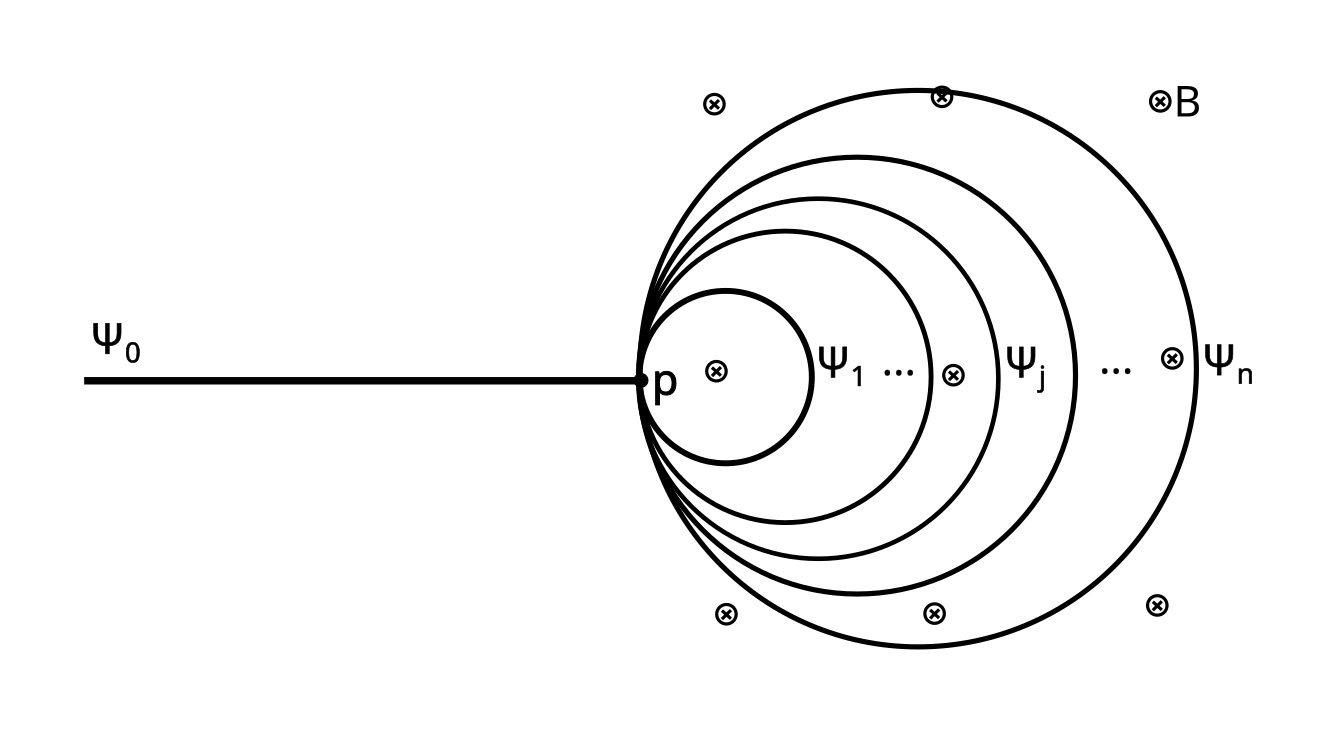
\includegraphics[width=12cm]{figs/intro_en/drawing}
\end{center}


\caption{\label{fig:draw}
Схема, изображающая систему анализа. Система состоит из $n$ колец из заранее определенного проводящего материала, соприкасающийся в точке $p$, с различными радиусами $R_j \leq 1,0$ мкм. Имеется дополнительный прямой входной провод, который входит в систему и соединяется с кольцами в точке их пересечения, а также поперечное магнитное поле $B$. Для каждого из $n$ колец определена волновая функция электронов $\psi_j$, а $\psi_0$ определяет волновую функцию входного провода. Для электрона на каждой из линий (рёбер графа) задаётся уравнение Шрёдингера, а в точке пересечения $p$ (узле графа) задаются граничные условия.
%A diagram depicting the system of analysis. Система состоит из $n$ колец of a predefined conducting material, соприкасающийся в точке $p$, с разными радиусами $R_j \leq 1,0$ $\mathrm{\mu m}$. There is an additional straight input lead, coming into the system and meeting the rings at their point of intersection, as well as a magnetic field $B$ perpendicular to the plane of the rings. For each of the $n$ rings, an electron wave function $\psi_j$ is defined, with $\psi_0$ defining the wave function of the input lead. A Schrodinger equation is defined for the electron on each of the lines (graph edges), while boundary conditions are defined at the point of intersection $p$ (the graph node). 
}
\end{figure}
\end{center}

Для анализа этой системы подходит баллистическая аппроксимация. Электрон движется с достаточно большой скоростью ($1,39 \times 10^6$ м/с) \citeph на достаточно малом расстоянии ($R \le 1$ мкм), поэтому взаимодействием электронов с окружающей средой можно пренебречь. Таким образом, квантовые графы \citeph являются достаточно точным приближением для определения уравнений движения и граничных условий.
%A ballistic approximation is suitable for the analysis of this system. The electron is traveling at large enough speeds ($1.39 \times 10^6 \frac{\mathrm{m}}{\mathrm{s}}$) \citeph for a small enough distance ($R \le 1\,\mathrm{\mu m}$), that the interaction between the electrons and their surroundings can safely be ignored. Therefore quantum graphs \citeph provide a reasonable approximation for defining the equations of motion and boundary conditions. 

Для каждой линии на графике (кольца и вход) строится одномерное уравнение Шрёдингера, определяющее волновую функцию электрона, который создает незатухающий ток. Затем в точке пересечения (узле графика) задаются граничные условия. Эти условия определяются законами Кирхгофа.
%For every line on the graph (the rings and the input) a one dimensional, time independent Schrodinger equation, determining the wave function of the electron which forms a persistent current there, is constructed. Boundary conditions are then defined at the point of intersection (the nodes of the graphs). These conditions are determined by Kirchhoff's circuit laws.

Ранее эта система была проанализирована для стандартного линейного уравнения Шрёдингера \citeph, и теперь мы хотим понять, что произойдет, если добавить в систему слабую нелинейность, моделирующую дополнительный потенциал самовзаимодействия.
%This system has previously been analyzed for the case of the standard linear Schrodinger equation \citeph, and we now wish to understand what happens if we add in a weak nonlinearity to the system, modeling an additional self-interaction potential. 
  
\subsection{Уравнение Шрёдингера}
Для начала предположим, что система находится в состоянии равновесия и является стационарной. Таким образом, этот анализ основывается на стационарном уравнении Шрёдингера. Хотя при определении собственных состояний нелинейной системы есть свои нюансы, в данном случае исследуемая система является слабо нелинейным, достаточно близкой к линеаризованному решению, и интересует, как нелинейность влияет на то, что уже известно. Поэтому для анализа определяются собственные состояния как собственные состояния известного решения линеаризованного уравнения. 
%здесь исследуемый объект является слабо нелинейным
%We start by assuming that we are in an equilibrium where the system is stationary. Thus this analysis will proceed with the time-independent Schrodinger equation. While there is a nuance in defining eigenstates for a nonlinear system, here the subject of interest is weakly nonlinear, sufficiently close to a linearized solution, and we are interested in how the nonlinearity changes what we know, so we define our subject of interest for analysis as the eigenstates of the known linearized solution.
Стационарное нелинейное уравнение Шрёдингера для колец определяется как
%The time independent nonlinear Schrodinger equation for our rings is defined as
\begin{equation}
\hat{H} \psi_j = k^2 \psi_j = \left(i\frac{d}{dx}+B\pi R_j \Phi_0^{-1}\right)^2\psi_j + \mu \frac{m_e}{\left|e\right| \hbar}\left|\psi_j\right|^2\psi_j
\end{equation}
где $j$ обозначает анализируемое кольцо. В этом уравнении 
$\Phi_0=\frac{2 \pi \hbar}{\left|e\right|}$ — квант магнитного потока, определяющий единицы измерения магнитного потока, а $\frac{m_e}{\left|e\right| \hbar}$ определяет единицы измерения $\mu$.
Физические константы: $\hbar$ -- приведённая постоянная Планка, $c$ -- скорость света, $m_e$ — масса электрона, $\left|e\right|$ — элементарный электрический заряд. Параметры: $k$ — волновое число электрона, $B$ — напряжённость магнитного поля, $R_j$ — радиус $j$-го кольца, $\mu$ — коэффициент электрон-электронного взаимодействия. Независимая переменная $x$ — это положение на кольце, отсчитываемое от точки пересечения против часовой стрелки. Зависимая переменная $\psi$ — это волновая функция электрона.
%where $j$ designates which ring is being analyzed. In this equation, 
%$\Phi_0=\frac{2 \pi \hbar}{\left|e\right|}$ is the magnetic flux quantum, defining the units of magnetic flux, while $\frac{m_e}{\left|e\right| \hbar}$ sets the units of $\mu$.
%The physical constants are $\hbar$ -- the reduced Planck constant, $c$ -- the speed of light, $m_e$ -- the mass of the electron, and $e$ -- the electric charge of the electron. The parameters are $k$ -- the electron wave number, $B$ -- the magnetic field strength, $R_j$ -- the radius of the $j$th ring, and $\mu$ -- the nonlinear coupling coefficient. The independent variable $x$ is the position on the ring, starting at the point of intersection and traveling counterclockwise. The dependent variable $\psi$ is the wave function of the electron.

Когда $\mu = 0$, нет электрон-электронного взаимодействия, 
и уравнение возвращается к линейному уравнению Шрёдингера (рассмотренному в \citeph). В этом случае членами уравнения являются стандартный кинетический член и члены, связанные с взаимодействием электрона с магнитным полем. Добавление члена с $\mu$ к уравнению добавляет потенциальный член для самовзаимодействия (электрон-электронного взаимодействия) в точке, определяя модель слабо нелинейной системы.
%and the equation returns to the linear Schrodinger equation (analyzed in \citeph). In this case, the terms are the standard kinetic term and the terms related to the interactions between the electron and the magnetic field. Adding $\mu$ adds a potential term for self interaction (electron-electron interaction) at a point, defining a model for a weakly nonlinear system. 
% When the term with mu is added to the equation, 

Предполагается, что уравнение Шрёдингра для электрона для входного провода является линейным и не содержит потенциала,
%The input is assumed to be linear, with no potential,
\begin{equation}
k^2 \psi_0 = -\frac{d^2}{dx^2}\psi_0,
\end{equation}
поскольку это не является целью данного анализа, а лишь требование системы.
%as it is not the desired subject of this analysis, just a requirement of the system.

Для полноты картины отметим, что с этими уравнениями связано несколько сложностей. Во-первых, единицы измерения $\hat{H}$ и $k^2$ не совпадают. Здесь изпользуются единицы измерения для $k^2$. Во-вторых, предполагается, что $\psi$ безразмерна. В линейном случае эти детали не имеют значения, поскольку $\psi$ можно умножить на любую константу без изменения уравнения. В нелинейном случае это не совсем так. Однако в нелинейном случае константа связи неизвестна, поэтому можно определить $\mu_{eff} = \mu_{true}\left|\psi\left(0\right)\right|^2$ и таким образом сохранить возможность изменять масштаб $\psi$ по своему усмотрению, если быть внимательным при выборе значения $\mu$.
%For completeness, there are a few complications with these equations. First the units of $\hat{H}$ and $k^2$ are not identical. Here we use the units for $k^2$. Second, $\psi$ is assumed to be dimensionless. In the linear case, these details are irrelevant as $\psi$ can be multiplied by an arbitrary constant without changing the equation. That is not quite true in the nonlinear case. However, the nonlinear case has an unknown coupling constant, so can define $\mu_{eff} = \mu_{true}\left|\psi\left(0\right)\right|^2$ and thus retain our ability to rescale $\psi$ at will as long as we are careful about our value of $\mu$.

При аналитических расчетах единицами измерения обычно пренебрегают, но в этой работе используется численный анализ, поскольку анализируемая система нелинейна. Поэтому очень важно соблюдать единообразие единиц измерения, даже если сами единицы могут быть любыми. При необходимости можно выполнить корректировку единиц измерения, умножив их на степени $m_e$, $c$, $\hbar$ и $\left|e\right|$, чтобы обеспечить единообразие. Первый пример, где возникает это требование — квант магнитного потока $\Phi_0$, в уравнении которого при использовании системы единиц СГС есть множитель $c$, отсутствующий в системе СИ.
%Units are typically ignored for exact calculations, but this work involves numerical analysis as the system of analysis is nonlinear. Therefore, consistency of units is very important even as the units themselves may not be. If required unit adjustments can be performed with by multiplying by powers of $m_e$, $c$, $\hbar$, and $\left|e\right|$, in order to ensure this consistency. The first such instance where this requirement appears is the magnetic flux quantum $\Phi_0$, where there is a factor of $c$ in the equation when solved with cgs units, which doesn't exist for SI units. 

\subsection{Граничные условия}
В точке пересечения есть два граничных условия.
%There are two boundary conditions at our point of intersection. 
Главные уравнения на границе (точке $p$) требует, чтобы значение $\psi$ для всех рёбер, пересекающихся в одной узле, было одинаковым,
%requires that the value of $\psi$ for all lines meeting at the point to be equal,
\begin{equation}
\psi_i\left(0\right) = \psi_i\left(2\pi R_i\right) = \psi_0\left(0\right) = \psi_j\left(0\right)  \text{ для } i \neq j
\end{equation}
%This is the equivalent of Kirchhoff's voltage law for quantum mechanics. 
%Note, that while the wave function is required to be continuous around the loop, its derivative is not such required at the point of intersection, due to the interaction between other rings and the input.
Это эквивалент правила напряжений Кирхгофа для квантовой механики.  
При этих правилах волновая функция должна быть непрерывной по всему ребру, но ее производная в узле не обязана быть непрерывной из-за взаимодействия между другими кольцами и входом.

%The second boundary condition is
Второе граничное условие является
\begin{equation}\label{eqn:kcl}
\frac{d\psi_0}{d x}\left(0\right) + \sum_{j=1}^n \left(-1\right)^{\sigma_j}\left(\frac{d}{dx}-iB\pi R_j \Phi_0^{-1}\right)\psi_j | _{x=0}= 0,
\end{equation}
где $\sigma_j = 0$ для исходящих рёбер и $\sigma_j = 1$ для входящих рёбер.
%where $\sigma_j = 0$ for outgoing lines and $\sigma_j = 1$ for incoming lines. \citeph
%\begin{equation}
%i k_0 \frac{r - 1}{r+1} = i \sum^{n}_{j = 1}k_j\left( a_j \left( 1 - e^{i \left(k_j + M_j\right) 2 \pi R_j} \right) - b_j \left( 1 - e^{i \left(-k_j + M_j\right) 2 \pi R_j}\right) \right).
%\end{equation}
Это эквивалент правила токов Кирхгофа для квантовой механики. Оно требует непрерывности производной на рёбрах графа, но не на его узлах.  
Поскольку наше уравнение Шрёдингера не зависит от значения $\psi\left(0\right)$, выбранного в точке, при условии, что соответствующим образом масштаб $\mu$ изменяется, как уже отмечалось ранее \citeph, это второе условие будет учитываться только при определении коэффициента отражения на входе. Это означает, что количество колец $n$ не влияет на относительный ток между кольцами. Таким образом, входной вывод $\psi_0$ необходим, поскольку в общем случае система не может соотвествовать уравнению
%This is the equivalent of Kirchhoff's current law for quantum mechanics. It requires continuity of the derivative on the graph edges, but not at the graph nodes. 
%Since our Schrodinger equation is invariant of the value of $\psi\left(0\right)$ chosen at the point as long as we appropriately rescale $\mu$, as previously observed \citeph, this second condition will only come into play when determining the reflection coefficient of the input. This means that the number of rings $n$ does not effect the relative current between the rings. The input lead, $\psi_0$, is thus required, as a general system can't satisfy Equation
\ref{eqn:kcl} где $\frac{d\psi_0}{dx}\left(0\right) = 0$ а $\psi_j \neq 0$.

%A final boundary condition will be added to this list -- 
В этот список будет добавлено последнее граничное условие —
\begin{equation}\label{eqn:psi0}
\psi\left(0\right) = 1.
\end{equation}
%This condition is our choice, as all of the previously given equations are invariant under this overall scaling, provided we properly rescale $\mu$. The equations only require that we choose a scale, it need not be the physical one. This choice is not the same choice as \citeph, where $\psi\left(0\right) = 1 + r$, $r$ being a reflection coefficient, determined from Equation \ref{eqn:kcl}. Neither choice are the physical one, as can be seen when we calculate current, but this fact is irrelevant, as we have merely rescaled our wave function. 
Это условие просто выбор, поскольку все приведенные выше уравнения инвариантны относительно этого общего масштабирования при условии, что масштаб $\mu$ изменили соответствующим образом. Уравнения требуют лишь выбор масштаба, который не обязательно должен быть физическим. Выбор, заданный уравнением \ref{eqn:psi0}, отличается от выбора в \citeph, где $\psi\left(0\right) = 1 + r$, где $r$ — коэффициент отражения, определяемый из уравнения \ref{eqn:kcl}. Ни один из этих вариантов не является физическим, что можно увидеть при расчете силы тока, но это не имеет значения, поскольку это отличие от физического выбора является просто изменением масштаба волновой функции.

\subsection{Параметры}
В отличие от работы Попова и др. \citeph, посколку этой анализ работает с численными вычислениями, требуются фактические значения всех параметров. В этом анализе пользует система единиц СИ. В большинстве исходных аналитических работ используются единицы СГС. В целом разница минимальна, но при пересчете единиц измерения нужно быть внимательным. Поскольку в этой работе рассматриваются электромагнитные свойства, 
следует учитывать, что в этих двух системах единицы измерения силы тока трактуются по-разному и их нельзя напрямую преобразовывать. 
%при преобразовании единиц измерения %нужно учитывать множитель скорость света, так как напрямую преобразовать единицы измерения нельзя.
%Due to the numerical nature of this analysis, unlike the case of Popov et. al. \citeph, here actual numbers for all parameters are required. This analysis will adopt the SI convention. Most of the source analyses use cgs units. In general, the difference is minimal, but one needs to be careful about rescaling units. Since this work involves electromagnetic properties, there is nuance in the conversion, and one needs to be careful of factors of the speed of light, as units are not directly convertible.
%Since this work involves electromagnetic properties, one needs to be careful of the fact that units related to current are treated differently in the two systems, and may not be directly convertible.
 
%The values of the parameters can be found from other sources. I will mostly be using them from an experiment by Chandrasekhar et. al. \citeph, as the experiment documented within includes rings of varying radius. This team used gold in their experiment, which is the reason why we have chosen gold for the material of the rings. 
Значения параметров можно найти в других источниках. В основном я буду использовать данные эксперимента Чандрасекара и др. \citeph, поскольку в эксперименте, описанном в статье, использовались кольца разного радиуса. Эта группа ученых использовала в своем эксперименте золото, поэтому мы выбрали золото в качестве материала для колец.

\subsubsection{$k$}

%The wave number is the Fermi wave number for our material, in this case gold. The Fermi energy is defined at absolute zero (our system is close to absolute zero in order to achieve a persistent current) defining the energy difference between the lowest and highest energy electrons at the ground state. It exists due to the Fermi exclusion principle. It effectively defines the minimum kinetic energy and velocity of electrons traveling in the conductor. \citeph
Волновое число — это волновое число Ферми для материала колец, в данном случае для золота. Энергия Ферми определяется при абсолютном нуле (наша система близка к абсолютному нулю, чтобы обеспечить постоянный ток) и представляет собой разницу энергий между электронами с наименьшей и наибольшей энергией в основном состоянии. Она существует благодаря принципу запрета Паули. По сути, она определяет минимальную кинетическую энергию и скорость электронов, движущихся в проводнике. \citeph

Для данного анализа значение $k$ установлено на уровне $1,20 \times 10^{10}$ м$^{-1}$. Это число указано в таблице как волновое число Ферми для золота. \citeph
%For this analysis, $k$ is set to $1.20 \times 10^{10}$ $\mathrm{m^{-1}}$. This number is given on a table as the Fermi wave number for gold. \citeph
%When I calculate the wave number I get a value twice this. The equation to calculate the Fermi wave number for non-interacting spin-$\frac{1}{2}$ particles is
%\begin{equation}
%\sqrt[3]{3\pi^2n}
%\end{equation}
%where $n$ is the electron density. [ref] The density of gold is known to be $19.3\, \frac{\mathrm{g}}{\mathrm{cm}^3}$. [ref?] This density will define the limits of our precision, as all other quantities are more precise. The atomic mass for gold is $196.9665 u$, and there are $79$ electrons per atom, so about $0.401$ electrons per atomic mass unit. We can thus calculate the electron density of gold 
%\begin{equation}
%n = \frac{N_A}{M}\rho n_{el}= \frac{6.02214076\times 10^{23} mol^{−1}}{196.9665 g/mol} 19.3 \frac{g}{cm^3} * 79 = 4.66 \times 10^{24} cm^{-3}
%\end{equation}
%This then gives us a Fermi wavenumber of
%\begin{equation}
%k_F = \sqrt[3]{3\pi^2\frac{N_A}{M}\rho n_{el}} = 2.40 \times 10^{10} m^{-1}
%\end{equation}
%Since factors of 2 are commonly lost in these calculations, I will use the value from the table.
%The choice of wave number is in some sense irrelevant. It will change the quantitative results but not the qualitative results. The wave number is also the only quantity dependent on the choice of material.
Выбор волнового числа в некотором смысле не имеет значения. Он повлияет на количественные, но не на качественные результаты. Кроме того, волновое число — единственная величина, зависящая от выбора материала.

\subsubsection{Ток}
%The numerical value of the current in a loop is unused, since for this analysis $\psi\left(0\right)$ is set to $1$. Typical values are on the order of $I_e \approx 10^{-7}$ A. If there is desire to understand the source of this number, one can roughly estimate the current produced by one electron traveling in a micrometer gold ring as
Численное значение силы тока в колце не используется, поскольку для данного анализа $\psi\left(0\right)$ приравнивается к $1$. Типичные значения составляют порядка $I_e \approx 10^{-7}$ А. Если вы хотите понять, откуда взялось это число, можно приблизительно оценить силу тока, создаваемого одним электроном, движущимся в золотом кольце микрометрового размера, как
\begin{equation}
I = \frac{e_e v_F}{R} = 3.54 \times 10^{-8} \mathrm{A}.
\end{equation}

\subsubsection{$R$}

Предполагается, что радиус колец варьируется от $0,57$ мкм до $1,0$ мкм. Для данного анализа мы примем значение $1,0$ мкм ($10^{-6}$ м) за $R_{max}$ и определим $R_j$ таким образом, чтобы радиус кольца составлял $R_j \, R_{max}$.
%The radii of the rings are assumed to vary from $0,57$ $\mathrm{\mu m}$ to $1,0$ $\mathrm{\mu m}$. For this analysis, we will define $1,0$ $\mathrm{\mu m}$ ($10^{-6}$ m) as $R_{max}$, and redefine $R_j$ such that the radius of a ring is $R_j \, R_{max}$. 

\subsubsection{$B$}
{\nprog 
Предполагается, что диапазон напряженностей магнитных полей находится в пределах
$1,5 \times 10^{-3}$ T$ < B < 1,30 \times 10^{-2}$ T. Значения B, выбранные Чандрасекаром и др., составляют 130 г, 120 г, 60 г, 30 г и 15 г. Насколько я понимаю, эти значения были выбраны таким образом, чтобы
%The range of magnetic fields strengths is assumed to fall within the range of
%$1,5 \times 10^{-3}$ T$ < B < 1,30 \times 10^{-2}$ T. The B values chosen by Chandrasekhar et. al. \citeph are 130 G, 120 G, 60 G, 30 G, and 15 G. My understanding is that these values were chosen so that 
\begin{equation}
\frac{B_{max}\pi R^2_{max}}{\Phi_0} = 1,
\end{equation}
%giving a single slow oscillation for $B = B_{max}$ and $R = R_{max}$. Our code has
выдает одно медленное колебание когда $B = B_{max}$ и $R = R_{max}$. В нашем коде
\begin{equation}\label{eqn:Boscil}
\frac{B_{max}\pi R^2_{max}}{\Phi_0} = \pi^2.
\end{equation}
%It turns out that these additional oscillations were required, or at the minimum useful, for the numerical analysis, and fitting a whole number of oscillations in a ring causes issues for certain calculations, while the results of this analysis show no issue with extrapolating the results for weaker magnetic field strengths. Therefore, this analysis retains the definition of $B_{max}$ given by Equation \ref{eqn:Boscil}. 
Оказывается, что эти дополнительные колебания были необходимы или, как минимум, полезны для численного анализа, и подгонка целого ряда колебаний к кольцу вызывает проблемы при определенных расчетах, в то время как результаты этого анализа не показывают проблем с экстраполяцией результатов для более слабых напряженностей магнитного поля. Следовательно, в этом анализе сохраняется определение $B_{max}$, данное уравнением \ref{eqn:Boscil}.

Обратите внимание, что сложность перевода между единицами измерения означает, что 1 Т эквивалентна 1000 Г, но не равна им из-за разницы в стандартах единиц измерения. Для единиц СИ,
%Note the complication of conversion between units means that $1$ T is equivalent to, but not equal to $1000$ G due to the difference in unit standards. For SI units, 
$\Phi_0^{-1}=\frac{\left|e\right|}{2 \pi \hbar}$. Использование СИ вместо СГС значит множителя $c$ в \citeph не будет.

%Throughout this analysis, $B$ is typically chosen in relation to $B_{max}$, instead of with respect to physical units. We also define a wave number 
В ходе этого анализа значение $B$ обычно выбирается по отношению к $B_{max}$, а не к физическим единицам измерения. Мы также определяем волновое число
%of the slow oscillations of the wave function (caused by the magnetic field).}
медленных колебаний волновой функции (вызванных магнитным полем),
\begin{equation}
M_j = \frac{B\pi R_j}{\Phi_0}.
\end{equation}
}


\subsubsection{Коэффициент нелинейности}

$\mu$ -- сила электрон-электронного взаимодействия. 
Поскольку мы предполагаем наличие нелинейности, а не выводим ее из теории, коэффициент нелинейности неизвестен. Поэтому значение $\mu$ подбирается таким образом, чтобы система оставалась в слабо нелинейном режиме. Значение $\mu$ должно быть достаточно большим, чтобы оказывать заметное влияние, но при этом достаточно малым, чтобы не создавать слишком много проблем. 

Уже известны некоторые свойства коэффициента нелинейности. Во-первых, в этой системе $\mu$ положительно, поскольку электроны отталкиваются друг от друга. Обратите внимание, что в данном случае электроны отталкиваются друг от друга не из-за электрического заряда, а из-за принципа запрета Паули, поскольку модель рассеяния нелинейного уравнения Шрёдингера описывает только точечные взаимодействия.   

Второе свойство заключается в том, что $\mu$ зависит от $\left|A\right|^{2}$. Поскольку $\psi\left(0\right)$ определён, как $\psi\left(0\right)=1$, все значения для $\mu$ относятся к $\mu_{eff} = \mu \left|\psi\left(0\right)\right|^2$. Поскольку $\psi\left(0\right)$ одинакова для всех колец, эта разница не имеет значения для данной системы.

Еще одно замечание по поводу изменения масштаба $\mu$. Ток $I_j = \left|a_j\right|^2 - \left|b_j\right|^2$ имеет те же единицы измерения, что и $\left|\psi\left(0\right)\right|^2$. Если приравнять $\psi\left(0\right)$ к чему-то порядка $\sqrt{I} \approx \sqrt{10^{-7}\, A}$, то потребуется изменить единицы измерения безразмерной на данный момент величины $\mu$, прежде чем ее можно будет использовать для оценки значения $\mu$.
%Since we propose non-linearity instead of deriving it, the nonlinearity coefficient is not known. $\mu$ is therefore chosen in order to remain in the weakly non-linear regime. $\mu$ should be large enough to have a noticeable effect, but small enough not to produce too many issues. 

%We already know a few properties about the nonlinearity coefficient. First, $\mu$ in our case is positive, as electrons repel each other. Note that in this case, technically the fact that electrons repel each other is due to the Pauli exclusion principle, not due to electric charge, since the scattering model of the nonlinear Schrodinger equation models point interactions only.  

%The second property is that $\mu$ зависит от $\left|A\right|^{2}$. Since we define $\psi\left(0\right)=1$, we keep in mind that all of our numbers for $\mu$ are actually for $\mu_{eff} = \mu \left|\psi\left(0\right)\right|^2$. Since $\psi\left(0\right)$ is the same for all rings, this difference is irrelevant for this system. 

%Another note of rescaling of $\mu$. The current $I_j = \left|a_j\right|^2 - \left|b_j\right|^2$ has the same units as $\left|\psi\left(0\right)\right|^2$. Setting $\psi\left(0\right)$ to something of the order of  $\sqrt{I} \approx \sqrt{10^{-7}\, A}$ requires rescaling the units of the currently dimensionless $\mu$ before it can be used to estimate the value of $\mu$.

\end{document}









